\documentclass[output=paper]{langsci/langscibook}
\author{Jeffrey Watumull\affiliation{Oceanit}\and Noam
    Chomsky\affiliation{University of Arizona, Massachusetts Institute of
Technology}}
\title{Rethinking universality}

% \chapterDOI{} %will be filled in at production

\abstract{For a discrete infinity of reasons, Ian Roberts is to be celebrated.
    Here we discuss how his important work has caused us to rethink what could
    be, arguably, the most unbelievable and extraordinary aspect of language:
    its \emph{universality}. In particular, we proffer Roberts’ theory of
parameter hierarchies to corroborate an \emph{Economy Thesis} -- a thesis
implying that the quiddities of language transcend \emph{human} language, and
would obtain of \emph{any} language \emph{anywhere} in the universe.}

\maketitle

\begin{document}\glsresetall

\section{Beyond the infinite}%\footnote{The scholarly odyssey of Ian Roberts merits the brilliance of Kubrickian flare.}

“As far as anyone knows, spaceships have been successfully built by exactly one
civilisation in the entire history of the universe: by post-1957 humans (the
Space Age actually happens to coincide exactly with my lifetime, although I had
nothing to do with it)” \citep[1]{Roberts2017}. Ian Roberts may not have been
amongst those to \emph{engineer} the Space Age, but he is one of the best to
have \emph{explained} (indirectly) how it was possible, and \emph{explanation}
is the prerequisite for all progress in scientific understanding and its
technological applications. Specifically, Roberts has over his career explained
how \emph{human} \emph{language}—its structure, acquisition\is{language acquisition}, and historical
change—has propelled our species to being the paragon of animals--to go
\enquote{beyond the infinite} in Kubrick's words. \blockquote{Chimps, who
    allegedly share around 98 percent of their genes with us, […] show no
    interplanetary ambitions[…]. Our extra 2 percent makes us extremely good—by
    the standards of everything else in the known universe, unbelievably,
    extraordinarily, \emph{cosmically} good—at generating, storing and
    transmitting knowledge. How do we do it? With \emph{language}.
\citep[1--2]{Roberts2017}} In this, the sixth decade of Roberts’ cosmic
existence, we celebrate him and how his work has caused us to rethink what
could be, arguably, the most unbelievable and extraordinary aspect of language:
its \emph{universality}. In particular, we proffer Roberts’ theory of
\isi{parameter hierarchies} to corroborate an \emph{Economy Thesis}—a thesis
    implying that the quiddities of language transcend \emph{human} language,
    and would obtain of \emph{any} language \emph{anywhere} in the universe.

\section{A universal instrument}

The human mind, Descartes argued, is undoubtedly in some sense a “universal
instrument”. We cannot know with certainty what he intended by this provocative
comment, but we do know that the Cartesians would have understood language as
fundamental to any nontrivial notion of “universality” because it is language
that empowers humans to generate an unbounded set of hierarchically structured
expressions that can enter into effectively infinitely many thoughts and
actions – that is, the competence of every human, but no beast or machine, to
use language in creative ways appropriate to situations but not caused by them,
and to formulate and express these thoughts coherently and without bound,
perhaps “incited or inclined” to speak in particular ways by internal and
external circumstances but not “compelled” to do so. Of course in the
pre-Turing world, the Cartesians did not know how a finite “machine” such as
the brain could generate the infinity of expressions of natural language, and
therefore posited a soul where we need only posit a neurobiological Turing
machine (obviously idealized with unbounded memory, etc.). Nevertheless
Descartes intuited the essence of Turing universality: “Only a spiritual entity
could achieve the limitlessness of interactive language, putting words together
in indefinitely many ways”, and to do so in ways that are “free” (i.e., not
compelled by internal or external conditions) and intelligible and appropriate
to situations, and to do so over an unbounded range in different domains. “Any
material machine must specialize: while a machine might do very well some of
the things people do, it would necessarily be unable to do others. Any part or
organ needed a particular configuration to achieve a task, and it was
impossible to have enough different parts with the requisite configurations in
a single machine to make it act in all the contingencies of life in the same
way that our reason makes us act.’ Only disembodied reason could be ‘a
universal instrument.’” \citep[63]{Riskin2017}. Of course the genius of Turing
was to discover that “[i]t is possible to invent a single machine which can be
used to compute any computable sequence”; he called this mathematical object,
appropriately, the “universal machine” \citep[243]{Turing1936}.

Linguistic competence (and especially its creative use), in concert with other
mental faculties, establishes the general intelligence necessary for the
evolutionary “great leap forward” of our species (see \citealt{Chomsky2016book}).
As \citet[182]{Roberts2017} conjects, “there might have been a crucial mutation
in human evolution which led, in almost no time from an evolutionary
perspective, from [humans living in] caves to [their creating knowledge of such
sophistication as to enable us to imagine and construct things as complex as,
say,] spaceships. It’s a plausible speculation that the mutation in question
was whatever it is that makes our brains capable of computing recursive syntax,
since it’s the recursive syntax that really gives language – and thought –
their unlimited expressive power. It’s one small step from syntax to
spaceships, but a great leap for humans”. A great leap for humans – and
\emph{only} humans, evidently (see \citealt{BerwickChomsky2016}). The
architecture of intelligence necessitates “provisions for recursive,
hierarchical use of previous results” as manifested in the “articulation” of a
complex structure into descriptions of “elementary figures” and “subexpressions
designating complex subfigures”, with a “figure first divided into two parts;
and then with each part described using the same machinery”
\citep[16]{Minsky1963}. The recursive capacity of intelligence is most manifest
in natural language: “Whatever we can express or describe, we can treat its
expression or description as though it was a single component inside another
description. In languages, this corresponds to using embedded phrases and
clauses. That final trick – of representing prior thoughts as things – gives
our minds the awesome power to use the same brain-machinery over and over
again, to replace entire conceptualizations by compact symbols, and hence to
build gigantic structures of ideas the way our children build great bridges and
towers from simple separate blocks. It lets us build new ideas from old ones;
in short, it makes it possible to think. The same is true of our [future]
computers” \citep[124]{Minsky1985}. Thus we might expect any
(super-)human-level intelligence anywhere in the universe – including any
genuine artificial intelligence (“our [future] computers”) we create – to be
recursive in this way.

It has been assumed that the essential properties of human language are not
only unique, but \emph{logically} \emph{contingent}:

\begin{quote}Let us define ‘universal grammar’ (\glsunset{UG}\gls{UG}) as the system of
principles, conditions, and rules that are elements or properties of all human
languages not merely by accident but by necessity – of course, I mean
biological, not logical necessity. Thus \gls{UG}\is{Universal Grammar} can be taken as expressing
\enquote{the essence of human language}. \citep[29]{Chomsky1975}
\end{quote}

“There is no \emph{a} \emph{priori} reason to expect that human language will
have such properties; Martian could be different” \citep[16]{Chomsky2000}.

This assumption, we submit, merits rethinking in light of Roberts’ work and
progress in the Minimalist Program more generally \citep{Chomsky1995}. Recent
work demonstrating the \emph{simplicity} \parencite{WatChoRob2017} and
\emph{optimality} \citep{ChoGalOtt2019} of language increases the cogency of
a conjecture that at one time would have been summarily dismissed as absurd:
“the basic principles of language are formulated in terms of notions drawn from
the domain of (virtual) conceptual necessity”, the domain defined by “general
considerations of conceptual naturalness that have some independent
plausibility, namely, simplicity, economy, symmetry, nonredundancy, and the
like” (\citealt{Chomsky1995}: 171, 1) that render linguistic computation
interestingly optimal. To the extent that this \emph{strong} \emph{minimalist}
\emph{thesis} (\glsunset{SMT}\gls{SMT})\is{Strong Minimalist Thesis} is true,
the essential – computational (even mathematical) – properties of language
would derive from laws of nature – language- and even biology-independent
principles that, once realized in the mind/brain, \emph{do} entail particular
properties as logically necessary. For instance, it is simply a fact of logic
that the simplest (optimal) form of the recursive procedure generative of
syntactic structures, Merge, has two and only two forms of application (i.e.,
external and internal).  Relatedly, \emph{given} the nature of the structures
\isi{Merge} generates, minimal structure distance is \emph{necessarily} the
simplest computation for the structure dependence of rules. And so on and so
forth (see \citealt{BerwickEtAl2011,Chomsky2013,Watumull2015} for additional
examples).

Research in the Minimalist Program starts with the optimality conjecture and
proceeds to inquire whether and to what extent it can be sustained given the
observed complexities and variety of natural languages. If a gap is discovered,
the task is to inquire whether the data can be reinterpreted, or whether
principles of simplicity and optimal computation can be reformulated, so as to
solve the puzzles within the framework of \gls{SMT},\is{Strong Minimalist Thesis} thus generating some support, in
an interesting and unexpected domain, for Galileo’s precept that nature is
simple and it is the task of the scientist to demonstrate it.

As we discover more and more of “the essence of human language” to be defined
by (virtual) conceptual necessity, the less and less absurd it is to question
just how contingent a phenomenon human language really is. It may well be with
language as with other phenomena studied in the natural sciences that, in the
words of the sage physicist J.A. Wheeler, “[b]ehind it all is surely an idea so
simple, so beautiful, that when we grasp it – in a decade, a century, or a
millennium – we will all say to each other, how could it have been otherwise?”
\citep[386]{Wheeler1986}. In other words, there may well be some \emph{a
priori} reasons to expect human language to have the (essential) properties it
does; or, to put it whimsically, the Martian language might \emph{not} be so
different from human language after all. In short, the \emph{universality} of
universal grammar needs to be rethought.

\section{Simplicity itself}

Our rethinking is based on a rethinking – or reminding – of \emph{simplicity}
as originally conceived in generative linguistics. “[S]implicity, economy,
compactness, etc.” were proffered in the first work on generative grammar as
criteria the grammar of a language must satisfy: “Such considerations are in
general not trivial or \enquote{merely esthetic}. It has been recognized of
philosophical systems, and it is, I think, no less true of grammatical systems,
that the motives behind the demand for economy are in many ways the same as
those behind the demand that there be a system at all” (\citealt{Chomsky1951}:
1, 67). This proposition echoed that of \citet[107]{Goodman1943}: “The motives
for seeking economy in the basis of a system are much the same as the motives
for constructing the system itself”. The idea is elementary but profound: if
the theory is no more simple, economical, compact, etc. than the data it is
proffered to explain, it is not a theory at all; hence the more compressed the
theory, the more successful – i.e., the more explanatory – it is.

The mathematician Gregory \citet[64]{Chaitin2005} has formalized this idea in
terms of algorithmic information theory: {“a scientific theory [can
be thought of] as a binary computer program for calculating observations, which
are also written in binary”; a generative grammar can thus be thought of as a
program for generating syntactic structures.}{} {“And you have a
law of nature if there is compression, if the experimental data is compressed
into a computer program”, equivalently a grammar, “that has a smaller number of
bits than are in the data that it explains”, or generates.}{~“}{The
greater the degree of compression, the better the law, the more you understand
the data.} {But if the experimental data cannot be compressed, if
the smallest program for calculating it is just as large as it is[...], then
the data is lawless, unstructured, patternless, not amenable to scientific
study, incomprehensible.} {In a word, random, irreducible”. In
the terms of generative grammar \parencite[285]{ChomskyMiller1963}: “As a
matter of principle, a grammar must be finite.}{} {If we permit
ourselves grammars with an unspecifiable set of rules[,] we can simply adopt an
infinite sentence dictionary.} {But that would be a completely
meaningless proposal.} Clearly, a grammar must have the status
of a theory about those regularities that we call the syntactic structure of
the language”. To have the status of a theory, the grammar must be compressed,
generating –and thereby explaining – the regularities in syntactic structures.

This idea is appreciated surprisingly seldom today: many computational
cognitive scientists and machine learning theorists (and hence virtually all
“artificial intelligence” (“AI”) labs in academia and industry) have perversely
redefined a successful theory or computer program to be one that merely
approximates or classifies unanalyzed data. This contrasts dramatically with
the Enlightenment definition in which data are selectively analyzed as evidence
for/against conjectured explanations (see
\citealt{Popper1963,Chomsky2000,Deutsch2011}). The machine learning systems
(e.g., deep learning neural nets, reinforcement learning techniques, etc.) so
popular in the current “AI spring” are \emph{weak} \emph{AI}: brute-force
systems laboriously trained to “unthinkingly” associate patterns in the input
data to produce outputs that approximate those data in a process with no
resemblance to human cognition (thus betraying Turing’s original vision for
AI). These systems will never be genuinely intelligent, and are to be
contrasted with the \emph{strong} – \emph{anthronoetic} – \emph{AI} Turing
envisioned: a program designed to attain human-level competence with a
\emph{human-style} typified by \emph{syntactic} \emph{generativity} and
\emph{semantic} \emph{fluidity} – to think \emph{the} \emph{way} a human
thinks. Today such programs,  based on generative grammars, are finally being
built.\footnote{\url{https://www.oceanit.com/science-technology/artificial-intelligence/}}

The early discussions on simplicity were addressing the logic of theory
construction by the scientist, but later \citep[4]{Chomsky1965} this logic was
analogized to the learning of language by children: “The problem for the
linguist, as well as for the child learning the language, is to determine from
the data of performance the underlying system of rules that has been mastered
by the speaker-hearer”. To determine the grammar (qua “theory” \emph{in} the
mind of the learner and qua theory \emph{of} the mind by the linguist), some
procedure to evaluate candidate grammars is necessary. Specifically, a
format-evaluation framework: “(v) specification of a function \emph{m} such
that \emph{m}(\emph{i}) is an integer associated with the grammar
G\emph{\textsubscript{i}} as its value (with, let us say, lower value indicated
by higher number)” \parencite[31]{Chomsky1965}. Naturally, “simpler” grammars are more
highly valued, but, then as now, “simplicity” is complex: “In the context of
this discussion, ‘simplicity’ (that is, the evaluation measure \emph{m} of (v))
is a notion to be defined within linguistic theory along with \enquote{grammar},
\enquote{phoneme}, etc. Choice of simplicity measure is rather like determination of
the value of a physical constant” \parencite[37--38]{Chomsky1965}.
\citet[107--108]{Goodman1943} too was cognizant of the \isi{complexity} of simplicity,
observing that “the mere counting of primitives is no satisfactory measure”
because “by the purely mechanical application of certain logical devices, we
can readily reduce all the primitives of any system to one”. Thus while Goodman
searched for a general notion of simplicity applicable to all systems, a
specific notion applicable to language was sought in generative linguistics,
and both ultimately “failed” (i.e., superseded by better notions—characteristic
of a healthy science): the former for technical reasons, the latter because of
the success of the Principles-and-Parameters (P\&P) framework
\citep{Chomsky1981}, which obviated the need for any simplicity measure of the
type envisioned for the format-evaluation framework.

\section{The Principles-and-Parameters mission}

\largerpage
In P\&P, language acquisition\is{language acquisition} is the process of setting the values for the
finitely many universal \isi{parameters} of the initial state of the language faculty
(\glsunset{UG}\gls{UG}). The apparent \isi{complexity} and diversity of linguistic phenomena is illusory
and epiphenomenal, emerging from the interaction of invariant principles under
varying conditions. This was a radical shift from the early work in generative
linguistics, which sought only an evaluation measure that would select among
alternative theories of a language (grammars) – the simplest congruent with the
format encoded in \gls{UG}\is{Universal Grammar} and consistent with the \isi{primary linguistic data}. But with
the P\&P shift in perspective, simplicity can be rethought, though this was
not initially appreciated. As discussed in the earliest work in generative
linguistics, notions of simplicity assume two distinct forms: the imprecise but
profound notion of simplicity that enters into rational inquiry generally, and
the theory-internal measure of simplicity that selects among I-languages. The
former notion of simplicity is language-independent, but the theory-internal
notion is a component of \gls{UG}, a subcomponent of the procedure for determining
the relation between experience and I-language (again, something like a
physical constant). In early work, the internal notion was implemented in the
form of the evaluation procedure to select among proposed grammars/I-languages
consistent with the \gls{UG}\is{Universal Grammar} format for rule systems. But, as Ian \citet{Roberts2012}
and others (e.g., \citealt{SheeBibRobHol2017}) discovered, the P\&P approach
transcends that limited, parochial conception of simplicity: with no evaluation
procedure, there is no internal notion of simplicity in the earlier sense.
There remains only the universal notion of simplicity.

In P\&P, grammars – I-languages – are simple, but, as evidenced in Roberts’
work (e.g., \citealt{RobHol2010}), they are so by virtue of
third-factor principles of computational efficiency \citep{Chomsky2005}, not by
analogy to theory-construction or by stipulation in \gls{UG}. In fact, rather than
“simple”, we propose to define P\&P-style acquisition\is{language acquisition} as “economical”, which,
in the Leibnizian spirit, we understand to subsume simplicity: “The most
economical idea, like the most economical engine, is the one that accomplishes
most by using least. Simplicity – or fuel consumption – is a different factor
from power [i.e., generative capacity, empirical coverage, etc.] but has to be
taken equally into consideration […]. The economy of a basis may be said to be
the ratio of its \emph{strength} to its simplicity. But superfluous power is
also a waste. Adequacy for a given system is the only relevant factor in the
power of a basis; and where we are comparing several alternative bases for some
one system, as is normally the case, that factor is a constant. Thus in
practice the simplest basis is the most economical” \citep[111]{Goodman1943}.
Economy, in other words, is a \emph{minimax} notion. In Leibniz’s words (see
\citealt{RobertsWatumull2015}): “the simplicity of the means counterbalances
the richness of the effects” so that in nature “the maximum effect [is]
produced by the simplest means”. This notion is enshrined in the Galilean ideal
(see \citealt{Chomsky2002}).

One economical form of P\&P-style learning explicable in terms of third-factors
is the traversal of a parameter hierarchy\is{parameter hierarchies} (see
\citealt{Roberts2012,Biberauer2016c}) – parameter specification. In such a
system, the child is not unthinkingly enumerating and evaluating
grammars.\footnote{Such an inefficient and unintelligent technique is the
\emph{modus} \emph{operandi} of many machine learning (weak AI) systems.}
Instead, the I-language matures to a steady state in a relatively deterministic
process of “answering questions” that \emph{emerge} \emph{naturally} \emph{and}
\emph{necessarily} in the sense that there exist “choices” in
acquisition\is{language acquisition} that logically must be “made” for the
system to function at all; none of the parameters need be encoded in the
genetic endowment (see \citealt{ObataEtAl2015} for similar ideas). This is the
ideal, of course. Like \gls{SMT}\is{Strong Minimalist Thesis} generally, how
closely it can be approximated is an empirical matter, and there remain many
challenges.

Parameter specification – i.e., the P\&P-conception of “learning”
as the specification of values for the variables in I-language – can be
schematized as a decision tree (parameter hierarchy) which, as Roberts has
shown, is governed by minimax economy: minimizing formal features
(feature-economy) coupled with maximizing accessible features
(input-generalization). Traversal of a hierarchy – a conditional-branching
Turing machine program – is inevitably economical in that the shortest (in
binary) and most general parameter settings are necessarily “preferred” in the
sense that the faster the computation halts, the shorter the parameter
settings. For instance, to specify word-order, a series of binary queries with
answers of increasing length and decreasing generality (microparameters) is
structured thus:

\begin{figure}

    \begin{tikzpicture}[baseline]

        \Tree 	[.{Is head-final present?}
                    [.{\fbox{\textsc{no}}}
                        {\textbf{head-initial}}
                    ]
                    [.{\fbox{\textsc{yes}}}
                        [.{Present on all heads?}
                            [.{\fbox{\textsc{yes}}}
                                \textbf{head-final}
                            ]
                                [.{\fbox{\textsc{no}}}
                                [.{Present on [+V] heads?}
                                    [.{\fbox{\textsc{yes}}}
                                        \textbf{head-final in clauses only}
                                    ]
                                    [.{\fbox{\textsc{no}}}
                                        {Present on \dots{}?}
                                    ]
                                ]
                            ]
                        ]
                    ]
                ]

    \end{tikzpicture}

\end{figure}

For compatibility with computability theory and Boolean logic, the parameter
hierarchy can be translated as follows:

\ea Hierarchy: \emph{H}
    \sn State \emph{T}: Decision Problem
    \sn Yes: 0/1 (0 = transition to state \emph{T}+1) (1 = halt and output parameter specification for \emph{H})
    \sn No: 0/1 (0 = transition to state \emph{T}+ 1) (1 = halt and output parameter specification for \emph{H})
\z

\ea Hierarchy: Word Order
    \sn State 1: Is head-final present?
    \sn Yes: Output 0 (transition to State 2)
    \sn No: Output 1 (halt and output “head-initial”)
    \sn {}
    \sn State 2: Present on all heads?
    \sn Yes: Output 1 (halt and output “head-final”)
    \sn No: Output 0 (transition to State 3)
    \sn {}
    \sn State 3: Present on [+V] heads?
    \sn Yes: Output 1 (halt and output “head-final in clause only”)
    \sn No: Output 0 (transition to State 4)
    \sn \dots{}
\z

So in P\&P, the logic is not “enumerate and evaluate” with stipulative
(theory-internal) simplicity measures: it is “compute all and only what is
necessary”, which implies the language-independent reality of economy in that,
as with the \isi{parameter hierarchies}, the process answers all and only the
questions it needs to. It is not that there is any explicit instruction in the
genetic endowment to prefer simple answers: it is simply otiose and meaningless
to answer unasked questions (i.e., once the \isi{parameters} are set, the computation
halts). (In this way it is trivial to derive Ockham’s razor from virtual
conceptual necessity. If the law of parsimony is not to multiple entities
beyond necessity, and language conforms to conceptual necessity, then ergo it
is maximally parsimonious. As \citet{Wittgenstein1922} observed: “Ockham’s
maxim is, of course, not an arbitrary rule, nor one that is justified by its
success in practice: its point is that unnecessary units in a sign-language
mean nothing” (5.47321); “If a sign is \emph{useless}, it is meaningless. That
is the point of Ockham’s maxim” (3.328).)

Moreover the “answers” to “questions” can be represented in binary. Indeed
binary is a \emph{notation-independent} notion necessary and sufficient to
\emph{maximize} computation with \emph{minimal} \isi{complexity}: functions of
arbitrarily many arguments can be realized by the composition of binary (but
not unary) functions – a truth of minimax logic with “far-reaching significance
for our understanding of the functional architecture of the brain”
(\citealt{GallistelKing2010}: \emph{x}). The mathematical and computational
import of binary was rendered explicit in the theories of \citet{Turing1936}
and \citet{Shannon1948}, the former demonstrating the necessarily digital –
hence ultimately binary – nature of \emph{universal} \emph{computation} (a
universal Turing machine being the most general mathematical characterization
of computation); the latter formalizing \emph{information} in terms of
\emph{bits} (binary digits). The consilience of these ideas is our Economy
Thesis: human language is based on simple representations (i.e., bits) and
strong computations (i.e., the binary functions of Turing machines) – and
“economy of a basis may be said to be the ratio of its \emph{strength} to its
simplicity” \citep[111]{Goodman1943}.

\section{Universal economy}

\largerpage
As one of the “general considerations of conceptual naturalness that have some
independent plausibility”, economy would be a factor that obtains of any
optimally “designed” (natural or artificial) computational system. So,
rethinking universality, if the Martian language were optimal in the sense of
conforming to virtual conceptual necessity, then it might be surprisingly
similar to human language. In point of fact, we ought not to be too surprised.
It is now well established by biologists that \emph{convergence} is a common
theme in any evolutionary process: “the number of evolutionary end-points is
limited: by no means is everything possible. [Because of evolutionary
convergence,] what is possible usually has been arrived at multiple times,
meaning that the emergence of the various biological properties is effectively
inevitable” (\citealt{ConwayMorris2013}: xii-xiii); indeed, the paleontologist
Simon Conway Morris argues that human-style intelligence was effectively
inevitable given the initial conditions of evolution on Earth. And there is no
reason \emph{a} \emph{priori} to assume that the principle of evolutionary
convergence is unique to the biology of a particular planet. Quite the
contrary, if we accept the rational form of inquiry in which the principle is
understood abstractly in a computational framework. The idea is that \emph{any}
computational system \emph{anywhere} made of \emph{anything} is governed by
\emph{laws} of computation. As the cognitive scientist C.R. Gallistel and
computer scientist Adam King argue persuasively
\parencite[167]{GallistelKing2010}:

\begin{quote}The functional structure of modern computers is sometimes discussed by
neuroscientists as if it were an accidental consequence of the fact that
computing circuits are constructed on a silicon substrate and communicate by
means of pulses of electrical current sent over wires. Brains are not
computers, it is argued, because computers are made of silicon and wire, while
brains are made of neurons. We argue that, on the contrary, several of the most
fundamental aspects of the functional structure of a computer are dictated by
the logic of computation itself and that, therefore, they will be observed in
any powerful computational device, no matter what stuff it is made of. In
common with most contemporary neuroscientists, we believe that brains are
powerful computational devices. We argue, therefore, that those aspects of the
functional structure of a modern computer that are dictated by the logic of
computation must be critical parts of the functional structure of brains
(\citealt[167]{GallistelKing2010})
\end{quote}

This argument simply reiterates \citeauthor{Turing1950}’s thesis
\parencite[446]{Turing1950} that “[i]f we wish to find such similarities [as
may exist between minds and machines] we should look [not at their substrates,
but] rather for mathematical analogies of function”.  And given this
universality of the functional, mathematical architecture of computation, it is
possible that we may need to rethink how uniquely human or even uniquely
biological our modes of mental computation really are. One interesting
implication is that we must rethink any presumptions that extraterrestrial
intelligence or artificial intelligence would really be all that different from
human intelligence.

So we assume that human language is a computational process that can be
characterized by a Turing machine (see \citealt{Watumull2015}). It is possible
to explore the space of all possible Turing machines (i.e., the space of all
possible computer programs), not exhaustively of course, but with sufficient
breadth and depth to make some profound discoveries. The late Marvin Minsky,
founder of the artificial intelligence laboratory at MIT, and his student
{Daniel Bobrow, once enumerated and ran some thousands of the
simplest Turing machines (computer programs with minimal numbers of rules).}{}
{Intriguingly, out of the infinity of possible behaviors, only a
surprisingly small subset emerged.} {These divided into the
trivial and the nontrivial.} {The boring programs either halted
immediately or erased the input data or looped indefinitely or engaged in some
similar silliness.} {The remainder, however, were singularly
interesting: \emph{all} of these programs executed an effectively
\emph{identical} counting function—a primitive of elementary
arithmetic.} {In fact, this operation reduces to a form of \isi{Merge}
(see \citealt{Chomsky2008}).} {More generally, these “A-machines”
(\emph{A} for \emph{arithmetic}) prove a point:}

\begin{quote}
    [I]t seems inevitable that, somewhere, in a growing mind some A-machines
    must come to be. Now, possibly, there are other, really different ways to
    count. So there may appear, much, much later, some of what we represent as
    ‘B-machines’ – which are processes that act in ways which are similar, but
    not identical to, how the A-machines behave. But, our experiment hints that
    even the very simplest possible B-machine will be so much more complicated
    that it is unlikely that any brain would discover one before it first found
    many A-machines. \parencite[121]{Minsky1985}
\end{quote}

\begin{quote}
    Let us think of this exploration as exposing parts of some infinite
    ‘universe of possible computational structures’. Then this tiny fragment of
    evidence suggests that such a universe may look something like
    [\Cref{fig:minsky}].\parencite[120]{Minsky1985}
\end{quote}

\begin{figure}
    \centering
    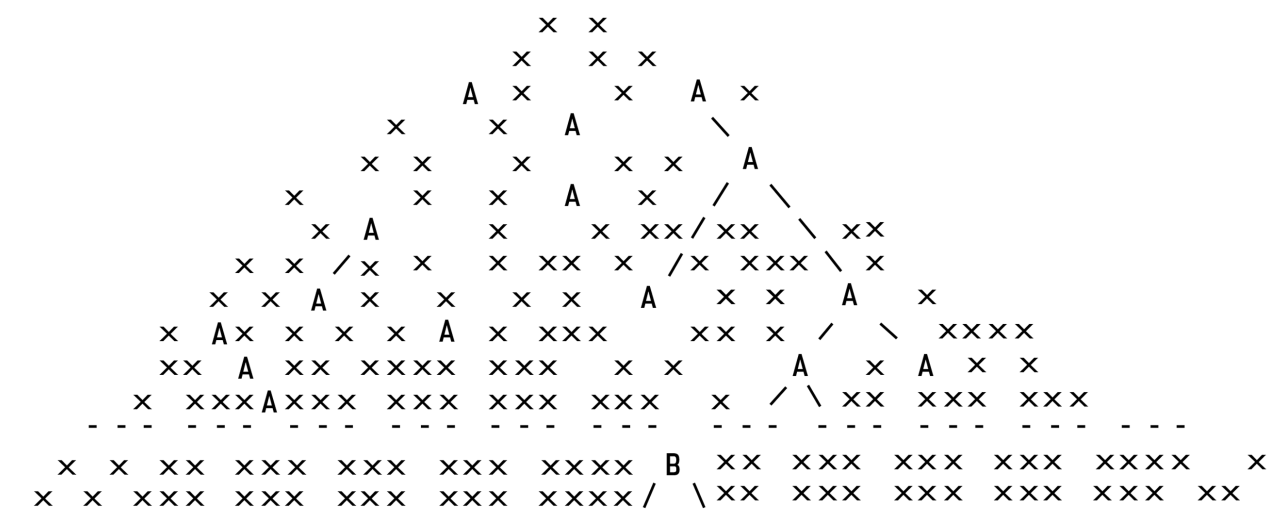
\includegraphics[scale=0.25]{./img/minsky}
    \caption{Representation of a universe with \enquote{A} and
        \enquote{B-machines}
    \parencite[120]{Minsky1985}}\label{fig:minsky}
\end{figure}

This is evidence that arithmetic – the foundation of any
mathematical/com\-pu\-tational system – as represented in an A-machine – reducible
to \isi{Merge} – is technically an \emph{attractor} in the \emph{phase space}
of possible mathematical structures: “any entity who searches through the
simplest processes will soon find fragments which do not merely resemble
arithmetic but \emph{are} arithmetic. It is not a matter of inventiveness or
imagination, only a fact about the geography of the universe of computation”
\citep[122]{Minsky1985}. Curiously, some physicists have argued that human
mathematics is contingent: “the next batch of aliens might turn out to be
different” \citep[774]{HutAlfordTegmark2006}, with no recognizable rules or
systems. This objection echoes once regnant dogma in linguistics that “[human]
languages could differ from each other without limit and in unpredictable ways”
such that linguists ought to proceed “without any preexistent scheme of what a
language must be” (\citealt{Joos1957}: 96, v), implying that any two human
languages could be as different from each other as any one could be from an
alien language. But this dogma could not withstand critical scrutiny, and was
dispelled with the advent of generative linguistics and its formulation of
universal grammar – the theory of the abstract grammatical system encoded
genetically in \emph{Homo sapiens sapiens} – and crucially by the deeper
empirical inquiries into the languages of the world undertaken within the
framework of generative grammar (e.g., the spectacular demonstration that
\ili{Warlpiri}, contrary to all appearances, has the standard hierarchical
structures universal to natural languages (see \citealt{Hale1976,Legate2001}).
To the extent that \gls{SMT}\is{Strong Minimalist Thesis} is true, general
properties derivative of this formal system define the properties universal to
particular languages.  Therefore we should indeed study these particular
languages with a “preexistent scheme of what a language must be” because
\gls{UG}\is{Universal Grammar} and general principles of computation constrain
the space of possible linguistic properties. And thus languages could not
“differ from each other without limit”, but only in “[predictable] ways”.

The thesis that arithmetic is an \emph{attractor} in the \emph{phase}
\emph{space} of possible mathematical structures obviously generalizes beyond
arithmetic to all simple computations (see \citealt{Wolfram2002} for countless
examples). “Because of this, we can expect certain ‘\emph{a} \emph{priori}’
structures to appear, almost always, whenever a computational system evolves by
selection from a universe of possible processes” \citep[119]{Minsky1985}.
Analogously, we submit that it is not implausible that an evolutionary search
through the simplest computations will soon find something like \isi{Merge}. \isi{Merge} is
an operation so elementary as to be subsumed somehow in every more complex
computational procedure: take two objects X and Y already constructed and form
the object Z without either modifying X or Y, or imposing any additional
structure on them: thus Merge(X, Y) = \{X, Y\}.\footnote{This formulation of
Merge requires some rethinking in ways that we can put aside here
(see~\citealt{Chomskyfc} for discussion).} This simple assumption suffices to derive in a
principled (necessary) way a complex array of otherwise arbitrary (contingent)
phenomena such as the asymmetry of the conceptual-intentional and sensory-motor
interfaces (entailing the locus of surface \isi{complexity} and variety), the
ubiquity of dislocation, \isi{structure-dependence}, minimal structural distance for
anaphoric and other construals, the difference between what reaches the mind
for semantic interpretation and what reaches the apparatus of articulation and
perception (see \citealt{Chomsky2017}).

\section{The dawn of language}

{As we discussed in terms of our Economy Thesis,} simplicity can
be defined in algorithmic information theory (or the theory of program-size
\isi{complexity}): the \isi{complexity} of a program is measured by its maximally
compressed length in bits so that the simplest program is that with the
shortest description. A search of the phase\is{phases} space of possible
programs, whether conducted consciously (e.g., by us, extraterrestrials, etc.)
or unconsciously (e.g., by modern computers, evolution, etc.) automatically
proceeds in size order from the shortest and increasing to programs no shorter
than their outputs (these incompressible programs are effectively lists); many
complex programs would subsume simpler programs as the real numbers subsume the
natural numbers. And, as demonstrated logically and empirically,
“any evolutionary process must first consider relatively simple systems, and
thus discover the same, isolated, islands of efficiency”
\citep[122]{Minsky1985}. Why are the simple systems (e.g., Merge) so sparsely
distributed in the phase\is{phases} space of possible processes? (Why are they
“islands”\is{islands}
in the computational universe?) Why are there no “similar” processes in the
neighborhood? (There is not something “like” arithmetic out there: there is
just arithmetic, “cold and austere, […] yet sublimely pure, and capable of a
stern perfection such as only the greatest art can show” in Bertrand Russell’s
words.) The answer must be that small sets of rules (e.g., Merge) can generate
unbounded \isi{complexity}, but the converse is not in general true: it is simply a
mathematical fact (a tautology) that there is only a small set of small sets of
rules, and thus not all complex phenomena can be generated by small sets of
rules (there is simply not a sufficient number of small sets of rules “to go
around”). This explains why, for instance, one cannot fiddle with arithmetic:
one cannot posit its simple rules, generate a universe of consequences, and
then make changes to that universe and expect the simple rules to cover the
“revised” universe (e.g., one cannot remove a number or change a sum, product,
etc.). Analogously, having posited \isi{Merge} and executed it to generate the
discrete infinity of syntactic structures, one cannot modify the logic (e.g.,
structure dependence) that obtains of those structures by dint of their having
been generated by \isi{Merge} and still expect \isi{Merge} to generate new structures that
conform to the modified logic, for the modified system is now “miraculous” in
the technical sense of possessing properties that did not emerge from the rules
themselves (or nonarbitrary third factors (i.e., laws of nature)). And there
cannot be infinitely many sets of small rules in the neighborhood of \isi{Merge} to
produce the effect of continuity. Thus there can only be~\emph{islands}~of
computation, not~\emph{continents}.\is{islands}

Thus it may well be that, given the universal and invariant laws of evolution,
convergence on systems – Turing machines – virtually identical to those
“discovered” in our evolutionary history is inevitable.\footnote{Indeed we
    might speculate that were we to “wind the tape of life back” and play it
    again, in Stephen Jay Gould’s phrasing, not only would something like \isi{Merge}
reemerge, but something like humans could well be “inevitable”, as some
biologists have suggested (see \citealt{ConwayMorris2013}).}  Hence our
rethinking the proposition “Martian could be different”.

The fact that simple computations are attractors in the phase\is{phases} space of possible
computations goes some way to explaining why language should be optimally
designed (insofar as \gls{SMT}\is{Strong Minimalist Thesis} holds) in that an evolutionary search is likely to
converge on it, which leads us to consideration of the origin of language.
Convergence is a consequence of constraints. As with intelligence, evolution
and development are possible only by coupling scope with constraints. Stated
generally: the scope of any creative process is a function of its operating
within limits. In the context of evolution, for instance, Stuart
\citet[118]{Kauffman1993} observes, “Adaptive evolution is a search process –
driven by mutation, recombination, and selection – on fixed or deforming
fitness landscapes. An adapting population flows over the landscape under these
forces. The structure of~such landscapes, smooth or rugged, governs both the
evolvability of populations and the sustained fitness of their members. The
structure of fitness landscapes inevitably imposes limitations on adaptive
search”. The analogy to mind is deeply nontrivial, for “intellectual activity
consists mainly of various kinds of search” \citep[431]{Turing1948}.

The evolution of language is mysterious (see \citealt{HauserEtAl2014}), but \gls{SMT}\is{Strong Minimalist Thesis}
is consistent with the limited archeological evidence that does exist on the
emergence of language, evidently quite recently and suddenly in the
evolutionary time frame (see \citealt{Tattersall2012}).\footnote{There is quite
    compelling evidence that since the trek of our ancestors from Africa some
    50,000 years ago, the language faculty has undergone no significant change,
    and not very long before (in evolutionary time) there is no evidence that
it existed at all.} Furthermore there is compelling evidence for \gls{SMT}\is{Strong Minimalist Thesis} in the
design of language itself. For instance, it is a universal truth of natural
language that the rules of syntax-semantics are \isi{structure-dependent} (see
\citealt{BerwickEtAl2011}): hierarchy, not linearity, is determinative in the
application of rules and interpretation of expressions. This implies a
far-reaching thesis with many consequences: linear order is a peripheral
property of language, emerging only in externalization at the sensory-motor
interface (where serial ordering is necessary). If this thesis holds generally,
then Aristotle’s dictum that language is “sound with meaning” should be
revised: language is not sound with meaning, but rather meaning with sound (or
some other modality of externalization), a very different concept, reflecting a
different traditional idea: that language is fundamentally an instrument of
thought – “audible thinking”, “the spoken instrumentality of thought”, as
William Dwight Whitney expressed the traditional conception (see
\citealt{Chomsky2013}), consistent with the Cartesian idea that language is a
central component of our mind as a “universal instrument”, endowing us with
general intelligence. As François Jacob suggested (see
\citealt{BerCho2011}), plausibly, “the role of language as a communication
system between individuals would have come about only secondarily” to the
emergence of generative syntax (Merge, we would now say) and its mapping of
structures to the conceptual-intentional system for semantic interpretation.
“The quality of language that makes it unique does not seem to be so much its
role in communicating directives for action” or other typical features of
animal communication, but rather “its role in symbolizing, in evoking cognitive
images”, in molding our notion of reality and yielding our capacity for thought
and planning, through its unique property of allowing “infinite combinations of
symbols” and therefore “mental creation of possible worlds”. Thus the most
reasonable speculation today – and one that opens productive lines of research
– is that from some simple rewiring of the brain, \isi{Merge} emerged, naturally in
its simplest form, providing the basis for unbounded and creative thought – the
“great leap forward” evidenced in the archeological record and in the
remarkable differences distinguishing modern humans from their predecessors and
the rest of the animal kingdom (see \citealt{Huybregts2017,BerwickChomsky2016}
for in-depth discussion of these topics).

If this conjecture can be sustained, we could answer the question why language
should be optimally designed: optimality would be expected under the postulated
conditions, with no selectional or other pressures operating; the emerging
system should just follow the laws of nature such as minimal computation and
more “general considerations of conceptual naturalness that have some
independent plausibility, namely, simplicity, economy, symmetry, nonredundancy,
and the like” – rather the way a snowflake forms. If this is correct, then,
contrary to what was once presumed, there \emph{would} be \emph{a}
\emph{priori} reasons to expect any language anywhere in the universe would
resemble human language; the “principles, conditions, and rules that are
elements or properties of all human languages” \emph{would} be \emph{logically}
necessary, deriving from laws of nature. And so, just as physicists seek “an
idea so simple, so beautiful, that […] we will all say to each other, how could
it have been otherwise?”, in the study of language we search for – and are
discovering – objects of great beauty and simplicity.

\section{The wonders of language}

\begin{quote}

It is […] quite possible that we, as a species, have crossed a cognitive
thre\-shold. Our capacity to express anything, through the recursive syntax and
compositional semantics of natural language, might have taken us into a
cognitive realm where anything, everything, is possible. Effectively, having
language has made us the equal of any extraterrestrial.
\parencite[181--182]{Roberts2017}

\end{quote}

Notwithstanding the universal logic of computation, it is obviously
necessary that there exist \emph{constraints} on the mind if it is to have any
\emph{scope} at all, and these constraints may very well be uniquely human.
Taking the extreme case, suppose that the human mind is a universal Turing
machine (see \citealt{Watumull2015}). Such a mind could be a \emph{universal}
\emph{explainer}. The argument is simple: a universal Turing machine can
emulate any other Turing machine (i.e., a universal computer can run any
program); a program is a kind of theory (written to be readable/executable by a
computer); thus a universal Turing machine can compute any theory; and thus,
assuming that everything in the universe could in principle be explained by and
understood within some theory or other (in other words, assuming no magic,
miracles, etc.), a universal Turing machine—a Turing-universal mind—could
explain and understand everything. It is an intriguing conclusion, and not
obviously false, but numerous objections could be posed. For instance, “an
arbitrary Turing machine, or an unrestricted rewriting system, is too
unstructured to serve as a grammar […]. Obviously, a computer program that
succeeded in generating sentences of a language would be, in itself, of no
scientific interest unless it also shed some light on the kinds of structural
features that distinguish languages from arbitrary, recursively enumerable
sets” \citep[360]{Chomsky1963}. Beyond language, if a
Turing-universal mind is to be a universal explainer, it should not generate
all possible explanations, true and false, because that would be merely to
restate the problem of explaining nature: deciding which in an infinite set of
explanations are the true (or best) explanations is as difficult as
constructing the best explanations in the first place. There must be “limits on
admissible hypotheses”, in the words of Charles Sanders Peirce (see
\citealt{Chomsky2006}). This interdependence of scope and limits has been
expounded by many creative thinkers and analyzed by (creative) philosophers of
esthetics: the beauty of jazz emerges not by “playing anything”, but only when
the improvisation is structured, canalized; the beauty of a poem is a function
of its having to satisfy the constraints of its form, as the mathematician
Stanislaw \citet[180]{Ulam1976} observed, “When I was a boy I felt that the
role of rhyme in poetry was to compel one to find the unobvious because of the
necessity of finding a word which rhymes. This forces novel associations and
almost guarantees deviations from routine chains or trains of thought. It
becomes paradoxically a sort of automatic mechanism of originality”. Thus from
science to art, we see that the (hypothesized) infinite creativity of the
Turing-universal human mind is non-vacuous and useful—and beautiful—only if it
operates within constraints – constraints that appear to be uniquely human.

\begin{quote}

    So understanding language means understanding a very big part of what it is
    to be human, what it is to be you. And that is perhaps the greatest wonder
    of language of all. \citep[182]{Roberts2017}

\end{quote}

The wonders of language Ian Roberts has illuminated are beyond counting; we
have surveyed but a twinkling here. Indeed, of his work we might say, in
closing, “my God!—\emph{it’s full of stars}!” \citep[202]{Clarke1968}.

\printchapterglossary{}

{\sloppy
\printbibliography[heading=subbibliography,notkeyword=this]
}

\end{document}

